\documentclass{acm_sen_article}

\usepackage{booktabs} % For formal tables
\usepackage{listings}
\usepackage{subfig}
\usepackage{url}
\usepackage{color}
\usepackage{authblk}
%\renewcommand{\baselinestretch}{0.99}

% Copyright
%\setcopyright{none}
% \setcopyright{acmcopyright}
%\setcopyright{acmlicensed}
% \setcopyright{rightsretained}
%\setcopyright{usgov}
%\setcopyright{usgovmixed}
%\setcopyright{cagov}
%\setcopyright{cagovmixed}


% DOI
% \acmDOI{10.475/123_4}

% ISBN
% \acmISBN{123-4567-24-567/08/06}

%Conference
% \acmConference[]{JPF Workshop}{Nov 2017}{Urbana-Champaign, IL USA}
% \acmYear{2017}
% \copyrightyear{2017}

%\acmPrice{15.00}


\begin{document}

\lstset{language=Java}

\lstdefinestyle{nonumbers}
{numbers=none}

\newcommand{\mike}[1]{\textcolor{red}{#1}}

\definecolor{mygreen}{rgb}{0,0.4,0}
\definecolor{mygray}{rgb}{0.5,0.5,0.5}
\definecolor{mymauve}{rgb}{0.58,0,0.82}
\lstset{ %
  backgroundcolor=\color{white},   % choose the background color; you
%must add \usepackage{color} or \usepackage{xcolor}
  basicstyle=\ttfamily\small,        % the size of the fonts that are used
%for the code
  basewidth = {.5em, 0.5em},
  breakatwhitespace=false,         % sets if automatic breaks should
%only happen at whitespace
  breaklines=true,                 % sets automatic line breaking
  captionpos=b,                    % sets the caption-position to bottom
  commentstyle=\color{mygreen},    % comment style
  deletekeywords={...},            % if you want to delete keywords from
%the given language
  escapeinside={\%*}{*)},          % if you want to add LaTeX within
%your code
  extendedchars=true,              % lets you use non-ASCII characters;
%for 8-bits encodings only, does not work with UTF-8
  frame=single,	                   % adds a frame around the code
  keepspaces=true,                 % keeps spaces in text, useful for
%keeping indentation of code (possibly needs columns=flexible)
  keywordstyle=\color{blue},       % keyword style
  language=C,                 % the language of the code
  otherkeywords={*,...},           % if you want to add more keywords to
%the set
  numbers=left,                    % where to put the line-numbers;
%possible values are (none, left, right)
  numbersep=5pt,                   % how far the line-numbers are from
%the code
  numberstyle=\tiny\color{black}, % the style that is used for the
%line-numbers
  rulecolor=\color{black},         % if not set, the frame-color may be
%changed on line-breaks within not-black text (e.g. comments (green
%here))
  showspaces=false,                % show spaces everywhere adding
%particular underscores; it overrides 'showstringspaces'
%  showstringspaces=false,          % underline spaces within strings
%only
  showtabs=false,                  % show tabs within strings adding
%particular underscores
  stepnumber=1,                    % the step between two line-numbers.
%If it's 1, each line will be numbered
  stringstyle=\color{mymauve},     % string literal style
  tabsize=2,	                   % sets default tabsize to 2 spaces
%  title=\lstname                   % show the filename of files included
%with \lstinputlisting; also try caption instead of title
  literate={->}{$\rightarrow$}{2}
           {α}{$\alpha$}{1}
           {δ}{$\delta$}{1}
}

\title{Veritesting Challenges in Symbolic Execution of Java}
\author[1]{Vaibhav Sharma}
\author[1]{Michael W. Whalen}
\author[1]{Stephen McCamant}
\author[2]{Willem Visser}
\affil[1]{University of Minnesota, Minneapolis, MN, United States of
America }
\affil[2]{University of Stellenbosch, Stellenbosch, South Africa}
\affil[1]{\textit {\{vaibhav,mwwhalen\}@umn.edu},
\textit{mccamant@cs.umn.edu}}
\affil[2]{\textit{wvisser@cs.sun.ac.za}}
% \author{Vaibhav Sharma}
% \affiliation{%
%   \institution{University of Minnesota}
%   \city{Minneapolis}
%   \state{MN}
%   \postcode{55455}
% }
% \email{vaibhav@umn.edu}
% 
% \author{Michael W. Whalen}
% \affiliation{%
%   \institution{University of Minnesota}
%   \city{Minneapolis}
%   \state{MN}
%   \postcode{55455}
% }
% \email{whalen@umn.edu}
% 
% \author{Stephen McCamant}
% \affiliation{%
%   \institution{University of Minnesota}
%   %\streetaddress{P.O. Box 1212}
%   \city{Minneapolis}
%   \state{MN}
%   \postcode{55455}
% }
% \email{mccamant@cs.umn.edu}
% 
% \author{Willem Visser}
% \affiliation{%
%   \institution{University of Stellenbosch}
%   \city{Stellenbosch}
%   \country{South Africa}
% }
% \email{wvisser@cs.sun.ac.za}
% \renewcommand{\shortauthors}{V. Sharma et al.}


\maketitle
\begin{abstract}
Scaling symbolic execution to industrial-sized programs is an important open research problem.
%
Veritesting is a promising technique that improves scalability by combining the advantages of static symbolic execution with those of dynamic symbolic execution.  The goal of veritesting is to reduce the number of paths to explore in symbolic execution by creating formulas describing regions of code using disjunctive formulas.
%
In previous work, veritesting was applied to binary-level symbolic execution.

Integrating veritesting with Java bytecode presents unique challenges,
notably, incorporating non-local control jumps caused by runtime polymorphism, exceptions, native calls, and dynamic class loading.
%
If these language features are not accounted for, we hypothesize that the static code regions described by veritesting are often small and may not lead to substantial reduction in paths.  We examine this hypothesis by running a Soot-based static analysis on six large open-source projects used in the Defects4J collection.
%
We find that while veritesting can be applied in thousands of regions, allowing static symbolic execution involving non-local control jumps amplifies the performance improvement obtained from veritesting.
%
We hope to use these insights to support efficient veritesting in Symbolic PathFinder in the near future.  Toward this end, we briefly address some engineering challenges to add veritesting into SPF.
\end{abstract}

%
% The code below should be generated by the tool at
% http://dl.acm.org/ccs.cfm
% Please copy and paste the code instead of the example below.
%
% \begin{CCSXML}
% <ccs2012>
%  <concept>
%   <concept_id>10010520.10010553.10010562</concept_id>
%   <concept_desc>Computer systems organization~Embedded systems</concept_desc>
%   <concept_significance>500</concept_significance>
%  </concept>
%  <concept>
%   <concept_id>10010520.10010575.10010755</concept_id>
%   <concept_desc>Computer systems organization~Redundancy</concept_desc>
%   <concept_significance>300</concept_significance>
%  </concept>
%  <concept>
%   <concept_id>10010520.10010553.10010554</concept_id>
%   <concept_desc>Computer systems organization~Robotics</concept_desc>
%   <concept_significance>100</concept_significance>
%  </concept>
%  <concept>
%   <concept_id>10003033.10003083.10003095</concept_id>
%   <concept_desc>Networks~Network reliability</concept_desc>
%   <concept_significance>100</concept_significance>
%  </concept>
% </ccs2012>
% \end{CCSXML}
%
% \ccsdesc[500]{Computer systems organization~Embedded systems}
% \ccsdesc[300]{Computer systems organization~Redundancy}
% \ccsdesc{Computer systems organization~Robotics}
% \ccsdesc[100]{Networks~Network reliability}

\keywords{multi-path symbolic execution; veritesting; Symbolic
PathFinder; static analysis}


\section{Introduction}
%Introduce veritesting, present our simple example and its performance improvement, segue into how veritesting at Java bytecode level is different from binary level
Symbolic execution is a popular testing technique that performs non-standard execution of a program.
%
Having been originally proposed in the 1970s, it has many applications
like test generation~\cite{dart,cute}, equivalence
checking~\cite{ramos,adaptorsynth}, finding
vulnerabilities~\cite{driller,angr}.%, checking correctness of transport protocols~\cite{transport}.
%
However, scalability continues to remain a challenge for symbolic execution.
%
Dynamic state merging~\cite{kuznetsov} provides one way to
alleviate scalability challenges by opportunistically merging dynamic
symbolic executors.
%
Veritesting~\cite{veritesting} is a different recently proposed
technique that is more suitable to symbolic execution tools that execute
one path at a time.
%
It has been shown to find more bugs, and achieve more node and path coverage, when implemented at the X86 binary level.
%
This provides motivation for investigating integration of veritesting with symbolic execution at the Java bytecode level.

Symbolic Pathfinder~(SPF)~\cite{spf} is a tool that performs symbolic execution of Java bytecode.
%
%SPF is tightly integrated with Java PathFinder~(JPF)~\cite{jpf} and uses JPF extensions to replace concrete execution with symbolic execution.
%
We present an example demonstrating the potential benefit of integrating veritesting with SPF in Listing~\ref{lst:v_ex}.
%
It checks if positive or negative integers occur more frequently in the
array~\textit{x}.
%
But, Listing~\ref{lst:v_ex} contains a hypothetical bug if \textit{x} contains an
equal number of positive and negative integers.
%
The three-way branch on lines 5, 6 causes the total number of execution
paths required to cover the \textit{for} loop to be $3^{\textit{len}}$.
%
However, this three-way branch can be combined into a multi-path region
and represented as a predicate by using disjunctions.
%
Each iteration through the loop can be represented by such a predicate.
%
\lstinputlisting[caption={An example to loop through a symbolic array with three execution paths through the loop body},
label={lst:v_ex}]{code_samples/VeritestingPerf.java}
%
\lstinputlisting[caption={SMT2 representation of multi-path execution in
Listing ~\ref{lst:v_ex} using \textit{len} = 2}, label={lst:v_ex_smt2}, language=lisp]{code_samples/ex.smt2.snippet}
%
We present such predicates in SMT2 notation in
Listing~\ref{lst:v_ex_smt2} assuming \textit{x} to contain two symbolic
integers named \textit{x0} and \textit{x1}~(\textit{len} equals 2).
%
The updates to \textit{sum} in the two loop iterations are captured by
\textit{sum0} and \textit{sum1}.
%
Using such predicates to represent the three-way branch on lines 5, 6 of
Listing~\ref{lst:v_ex} allows us to have only one execution path through
the loop body.
%
Figure~\ref{fig:v_ex_plot} shows a comparison of the number of execution
paths explored to find the bug on line 11 of Listing~\ref{lst:v_ex}.
%
The exponential speed-up from our predicates, representing a multi-path
region, allows us to find
the bug using just three test cases.
%
Veritesting provides a way to get such performance improvements by using
static analysis to identify multi-path
regions and create predicates to represent them.
%
\begin{figure}[]
\caption{Comparing number of execution paths from Listing~\ref{lst:v_ex} using vanilla SPF and SPF with static unrolling}
\label{fig:v_ex_plot}
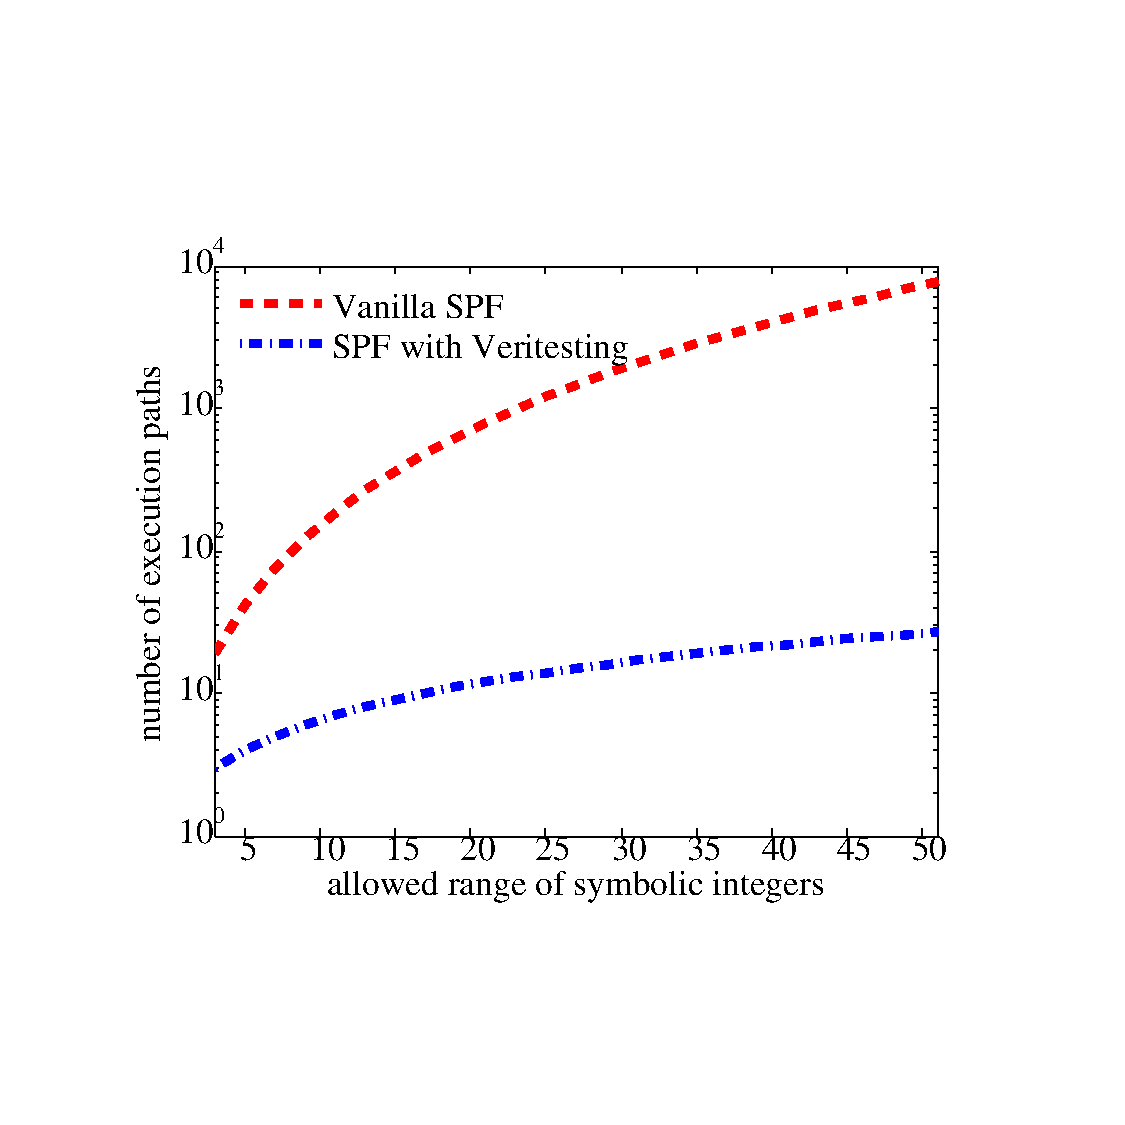
\includegraphics[width=\columnwidth]{figures/veritesting_example_semilogy}
\end{figure}
%

\section{Challenges}

While the performance improvement demonstrated on the code in Listing 1 is impressive, it is perhaps not representative of most Java code.  Java conventions encourage the use of indirection when accessing class fields using non-static {\em get} and {\em set} methods, as well as liberal use of exceptions.  Unlike C compilers, which assume a ``closed world'' and often inline simple functions into the body of calling methods to improve performance, the Java compiler must assume an ``open world'' in which a class may be used in a new context, so inlining of non-final methods is unsafe.  

Previous approaches to veritesting exit static code regions when indirect calls to functions or non-local jumps are made.  In this section, we explore how the structure of Java programs might reduce the performance of a n\"aive veritesting approach.

%Talk about how veritesting is different when done on Java bytecode
%
%The transition points at the Java bytecode level are return, exceptions (done using athrow), virtual function invocations (invokevirtual, invokeinterface), native calls (also done using invokevirtual), reflection and dynamic class loading (also done using invokevirtual).
%
%Present results from Soot-based static analysis
%
%Talk about how veritesting gets harder to do when considering multi-threaded Java bytecode.
\subsection{Exit Points}
\label{sec:exit_points}
%While the performance improvement shown in Figure~\ref{fig:v_ex_plot} with statically unrolling the three-way branches is clear, we need to automate this process.
%
Integrating veritesting with SPF requires that we can represent a region of a java program as a disjunctive formula with multiple exit points.  Each exit point describes a possible distinct continuation of the current path after the static code region completes execution.  Avgerinos et al.~\cite{veritesting} defined exit points as unresolved jumps, function boundaries, and system calls.
%
These exit points are nodes in a Control Flow Graph~(CFG) which represent non-local control flow, and therefore, need to be explored using plain dynamic symbolic execution.
%
In the context of Java bytecode, we find such non-local control flow in five ways listed as follows: (1) return statements, (2) exceptions, (3) virtual function invocations~(\textit{invokevirtual}, \textit{invokeinterface}), (4) reflection, (5) native calls.
%
Return statements form the function boundary, and are obvious candidates to be considered as exit points.
%
Exceptions are used to catch unexpected behavior, and often help design of cleaner code, and allow developers to capture useful information when such errors occur.
%
Virtual function invocations occur due to runtime polymorphism supported by Java.
%
The runtime environment binds the method call to its body by using the type of the object making the call.
%
Using reflection requires loading a class at runtime, identifying a method within the class, and calling it.
%
It is primarily used for extensibility purposes, achieving separate compilation, and generating a class at runtime.
%
An approach such as Avgerinos et al.~\cite{veritesting} would force
static code regions when any of these five constructs are encountered.

%Such regions must correctly preserve the semantics of symbolic execution for all possible Java constructs.
%
The primary benefit of implementing veritesting comes from its conversion of branches into disjunctions.
%
But this benefit exists only when the number of different exit points from the disjunctive formula is less than the number of execution paths through the region in the first place.
%
For example, all execution paths in the first three-way branch in
Listing~\ref{lst:v_ex} joined together on line 14, causing the three-way branch to have a single exit point.
%
Therefore, it is crucial for us to study the number of exit points for each of our statically-analyzed regions vs. the reduction in the number of branches within the region.
%
%
%Native calls are used to execute code outside of the Java Runtime Environment.
%
%Incorporating these into our static analysis would require handling virtual function invocations as well as static analysis of binary code.

These five types of exit points create the kind of non-local control flow which formed the frontier of the visible CFG created as a result of \textit{CFGReduce} step by Avgerinos et al.
%
However, many of these exit points are used pervasively by Java developers.
%
For example, the Visitor design pattern is used extensively by the ASM framework~\cite{asm}, Soot~\cite{soot} and makes use of Java\rq s dynamic dispatch mechanism.
%
Running into exit points too often causes our statically-analyzed regions to be small and our performance gain from having fewer branches to be lost.

We investigated the occurrence of these exit points further by creating a Soot-based static analysis of six large open-source projects written in Java.
%
Software faults from these six projects are maintained in the Defects4J~\cite{defects4j} repository.
%
We used Soot to create a CFG for every method body in every class file in these six projects.
%
For each CFG, we used nodes corresponding to \textit{if} bytecode instructions as a starting point of our analysis.
%
We measured the number of instructions encountered when traversing down each side of the branch until we get to the immediate post dominator~\cite{dragon-book} of our starting point.
%
If there were no exit points encountered on any side of the branch, we considered this region as a pure veritesting region and calculated its size in bytecode instructions.
%
Finally, we allowed upto five nested branches and calculated the number of bytecode instructions from the earliest, as well as, the latest starting point in our CFG traversal to an exit point.
%
We report our results in Tables~\ref{t:r_s} and~\ref{t:r_c}.
%
\begin{table}[]
\centering
\begin{tabular}{|l|l|l|l|l|l|}
\hline
        & \#classes & \begin{tabular}[c]{@{}l@{}}if-\\ return\end{tabular} & \begin{tabular}[c]{@{}l@{}}if-\\ invokevirtual\end{tabular} & \begin{tabular}[c]{@{}l@{}}if-\\ throw\end{tabular} & \begin{tabular}[c]{@{}l@{}}region \\ size\end{tabular} \\ \hline
chart   & 679       & 8.44                                                 & 27.47                                                       & 4.33                                                & 13.59                                                  \\ \hline
closure & 1339      & 7.35                                                 & 22.1                                                        & 9.5                                                 & 11.66                                                  \\ \hline
lang    & 170       & 6.70                                                 & 11.64                                                       & 7.09                                                & 9.60                                                   \\ \hline
math    & 1104      & 18.27                                                & 56.61                                                       & 9.56                                                & 27.06                                                  \\ \hline
mockito & 382       & 6.02                                                 & 12.51                                                       & 8.05                                                & 13.57                                                  \\ \hline
time    & 209       & 7.79                                                 & 13.10                                                       & 7.08                                                & 8.10                                                   \\ \hline
\end{tabular}
\caption{Soot-based analysis for number of bytecode instructions between starting and exit points}
\label{t:r_s}
\end{table}
%
\begin{table}[]
\centering
\begin{tabular}{|l|l|l|l|l|}
\hline
        & \begin{tabular}[c]{@{}l@{}}if-\\ return\end{tabular} & \begin{tabular}[c]{@{}l@{}}if-\\ invokevirtual\end{tabular} & \begin{tabular}[c]{@{}l@{}}if-\\ throw\end{tabular} & \begin{tabular}[c]{@{}l@{}}region\\ count\end{tabular} \\ \hline
chart   & 1712                                                 & 7760                                                        & 521                                                 & 6627                                                   \\ \hline
closure & 3853                                                 & 7466                                                        & 138                                                 & 9258                                                   \\ \hline
lang    & 3602                                                 & 1589                                                        & 539                                                 & 2065                                                   \\ \hline
math    & 2219                                                 & 5582                                                        & 662                                                 & 15375                                                  \\ \hline
mockito & 372                                                  & 572                                                         & 15                                                  & 574                                                    \\ \hline
time    & 1202                                                 & 984                                                         & 204                                                 & 1421                                                   \\ \hline
\end{tabular}
\caption{Number of occurences in Soot-based static analysis}
\label{t:r_c}
\end{table}
%
Table~\ref{t:r_s} shows the average size and Table~\ref{t:r_c} shows the number of times each such count was reported.
\mike{We need to explain these tables better: can we take a small code fragment (say, that of Listing 1) and explain it according to these numbers, or create a very tiny code fragment that demonstrates them?}
%
The \textit{if-return}, \textit{if-invokevirtual}, \textit{if-throw} columns in Table~\ref{t:r_s} report the average number of instructions observed between any \textit{if} opcode-containing bytecode instruction and a \textit{return}, \textit{invokevirtual} or \textit{invokeinterface}, \textit{throw} opcode-containing bytecode instruction.
%
These same columns in Table~\ref{t:r_c} report the number of times we observed an occurence of one of \textit{return}, \textit{invokevirtual}, \textit{invokeinterface}, \textit{throw} opcode-containing bytecode instructions before reaching the immediate post-dominator of the starting \textit{if} node on any side of the branch.
%
Tables~\ref{t:r_s} and~\ref{t:r_c} show that while we discover thousands of regions which do not contain any exit points, these regions are small.
%
They also show that early \textit{return} instructions are another often used construct in Java.
%
Having veritesting for these regions alone would provide a significant performance boost to SPF.
%
Table~\ref{t:r_c} shows \textit{invokevirtual} or \textit{invokeinterface} instructions are encountered far more often than \textit{return} or \textit{throw} instructions.
%
This can be explained by the pervasive use of runtime polymorphism and exception handling by Java developers.
%
Instead of using \textit{invokevirtual} and \textit{invokeinterface}
instructions as exit points, if we can continue our predicate
construction for multi-path regions beyond them, we would almost double
the number of veritesting regions in many cases.
%
\section{Engineering Challenges}
Research challenges such as static analysis of exit points and veritesting in a multi-threaded context need to be solved for integrating veritesting with any bytecode-level symbolic execution engine.
%
Symbolic PathFinder is a popular Java bytecode-level symbolic execution tool.
%
It has been used to find bugs in flight software~\cite{pasareanu2008}, to test large web applications~\cite{fujitsu}, and for testing Android apps~\cite{android_spf}.
%
It has also been extended for parallel symbolic execution~\cite{parallel}, and for load testing~\cite{load_testing_spf}
%Talk about the engineering challenges we face when implementing veritesting with Symbolic PathFinder
%
Given the large and diverse set of applications that stand to benefit from integrating veritesting with SPF, we discuss here the engineering challenges expected with such an integration.

\subsection{Shared Sub-expressions} 
%Sharing implementation needs to be fixed. Show this using the TestSharing example
Consider the code shown in Listing~\ref{lst:sharing}.
%
\lstinputlisting[caption={An example with an increasing formula size with every loop iteration}, 
label={lst:sharing}]{code_samples/TestSharing.java}
%
The function \textit{testSharing} adds the value of \textit{x} to itself in every loop iteration on line 3 of Listing~\ref{lst:sharing}.
%
The number of loop iterations is controlled by a user-supplied value for \textit{bound}.
%
On line 4, the code branches on the value of the value of \textit{x}.
%
We symbolically executed the \textit{testSharing} method with \textit{x} set to be symbolic and \textit{bound} set to be a concrete value.
%
We set the minimum and maximum symbolic integer values to be -100 and 100 respectively.
%
We increased the value of \textit{bound} from 1 to 29 and recorded the time taken and maximum memory used for complete path coverage.
%
Figure~\ref{fig:sharing_time} shows the trend seen for increasing values of \textit{bound}.
%
\begin{figure}[]
\caption{Time required for covering paths in Listing~\ref{lst:sharing} with increasing values for \textit{bound}}
\label{fig:sharing_time}
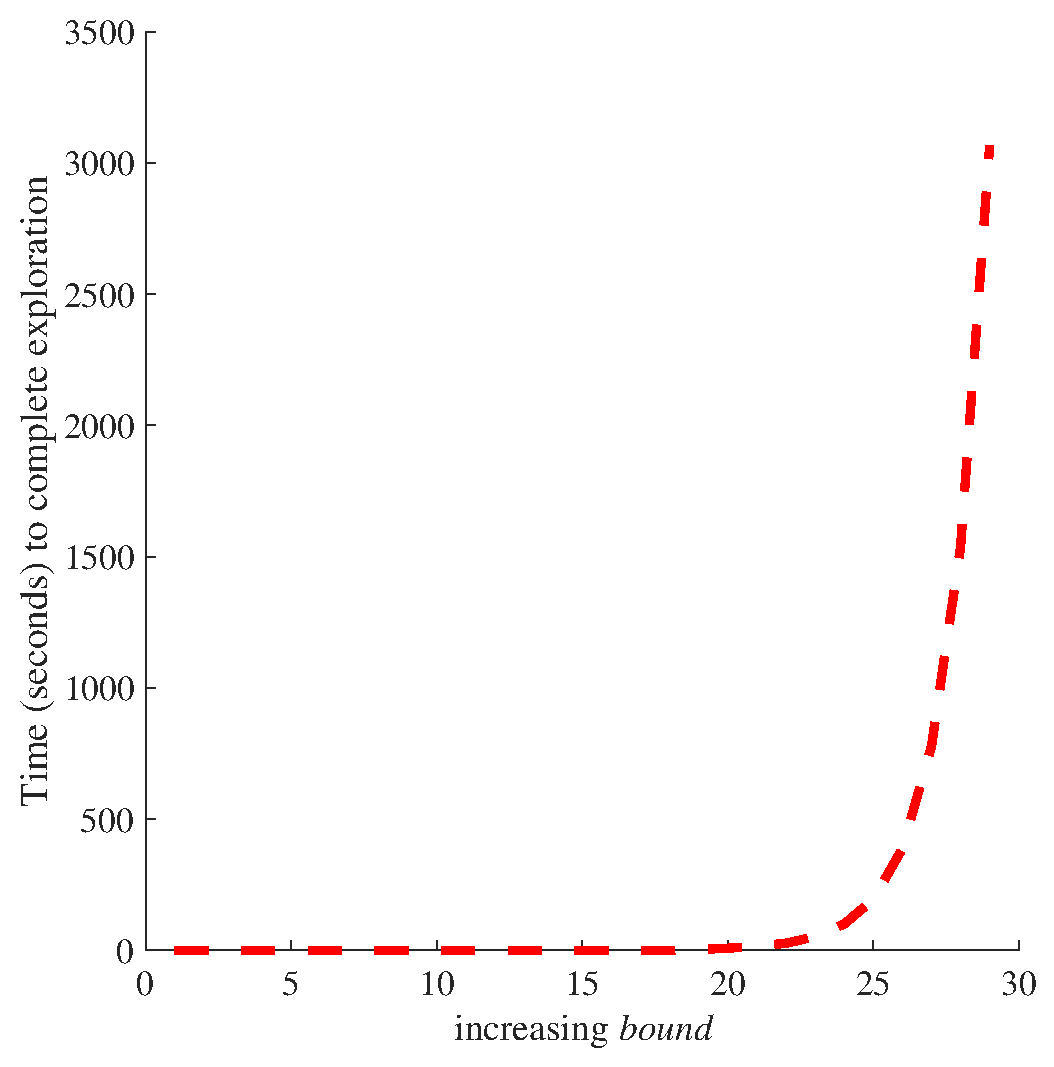
\includegraphics[width=\columnwidth]{figures/sharing_time}
\end{figure}
%
Figure~\ref{fig:sharing_time} shows that the running time remains constant until the value for \textit{bound} is 18, and then starts to rise exponentially.

\subsection{Complex Expressions}
Engineering issue \#2: Need to have complex expressions, talk about how Comparators cannot be used anywhere below the top-level operator

\subsection{Intermediate variables}
Engineering issue \#3: Nice to introduce intermediate variables

%
%
% \subsection{Veritesting with Multi-threading}
% Veritesting requires SPF to be able to perform static symbolic execution on a region of code and incorporate it as a disjunctive predicate into its path expression along with the corresponding updates to its symbolic store.
% %
% If the region being statically analyzed can be executed in a multi-threaded context, however, then it is necessary to consider all possible points of interference in the region.
% %
% This consideration requires changes to the updates made to SPF\rq s path expression and its symbolic store.
% %
% One way to handle this is to turn every point of interference as an exit point, but determining the possible points of interference statically is itself a difficult problem.  Likely it will require some level of dynamic analysis to determine the points of interference at the time of creation of a veritesting region.
% %
% %But, veritesting would be beneficial if its static analysis also includes computation of points at which interference is infeasible.
% %
% This makes creating an efficient veritesting approach challenging since the cost of this computation must be less than the cost of doing plain dynamic symbolic execution.
















% Data from perl script-based static analysis
% this script just counted the difference between instructions
%
% \begin{table}[]
% \centering
% \caption{My caption}
% \label{my-label}
% \begin{tabular}{|l|l|l|l|}
% \hline
%         & if-ret & if-IV & if-throw \\ \hline
% Chart   & 8.08   & 5.79  & 6.10     \\ \hline
% Closure & 7.40   & 4.37  & 12.6     \\ \hline
% Lang    & 6.3    & 5.23  & 8.26     \\ \hline
% Math    & 12.9   & 6.9   & 9.09     \\ \hline
% Mockito & 8.5    & 4.38  & 11.39    \\ \hline
% Time    & 9.0    & 5.56  & 9.3      \\ \hline
% \end{tabular}
% \end{table}

\section{Implementing Veritesting for Java}
In order to implement veritesting for SPF, we are leveraging existing tools and framework features within SPF.  The trickiest implementation aspects involve determining the bounds of static code regions over Java bytecodes and the mechanism for switching from ``standard'' symbolic execution using the SPF {\em SymbolicListener} class to one that can evaluate these multipath code regions. We briefly describe our prototype implementations for these aspects.
%
\subsection{Soot-based analysis for veritesting}
%
Veritesting requires static construction of
predicates of a multi-path region which represent changes to the path expression of the dynamic
symbolic executor.
%
It also requires construction of a control-flow graph of method bodies
from Java bytecode and finding exit points of the region, which in turn
requires creation of a control-flow graph of the region.
%
Implementing veritesting is made simpler by using a static single
assignment~(SSA)~\cite{ssa} representation of the multi-path region.
%
Using an SSA form allows us to use the $\phi$-expressions created by the
SSA form and translate them into points at the end of the veritesting
region where updates to system state along different paths in the region
can be merged.
%
Soot~\cite{soot} is a static analysis framework for Java programs that
has both these features, with
ExceptionalUnitGraph~\cite{exceptionalunitgraph} and the Shimple
IR~\cite{shimple}.
%
For simple regions with only one exit point, like the one presented in Listing~\ref{lst:v_ex}, we
were able to use Soot to automate static construction of the predicate representing
an update to the expression.
%
For doing this, we used nodes with more than one successor as the
starting point, found the immediate post-dominator of the starting
point, and traversed the control-flow graph on all sides of such branches.
%
During such a traversal, we constructed predicates representing the
multi-path region, similar to the ones presented in
Listing~\ref{lst:v_ex_smt2}.
%
As explained in Section~\ref{sec:exit_points}, including virtual
function invocations in the construction of our predicates amplifies the
benefits of veritesting even further.
%
We plan to automate this inclusion in the future using Soot.
%
Providing SPF with updates to be made to its symbolic store also
requires Soot to maintain stack location information for variables.
%
We plan to automate SPF\rq s symbolic store updates using Soot in the
future.
%
\subsection{Integrating Veritesting with Symbolic PathFinder}
%
Integration of veritesting requires changing Symbolic PathFinder so that it can 
use a Soot-based analysis.
%
We present the sequence of actions SPF must take to implement veritesting in 
Figure~\ref{fig:spf_veritesting}.
%
The source code in Listing~\ref{lst:v_ex} was modified to add a {\tt else return;} 
statement on line 7 to create the Java bytecode shown in Figure~\ref{fig:spf_veritesting}. 
%
This integration assumes our prior Soot-based analyis provides SPF 
with a table that maps instruction offsets~(representing the start of a 
veritesting region) to a set containing (1) the multi-path region predicate to be 
added to the path expression as a conjunction, (2) symbolic store
updates, (3) exit points, (4) the expression to branch on to one of the exit points.
%
Using SPF\rq s listener mechanism, we add a listener~(named SMPListener in Figure~\ref{fig:spf_veritesting}) which listens for instructions that are starting points for a Symbolic Multi-Path~(SMP) region.
%
On finding such an instruction, \textit{SMPListener} 
(1) updates the path expression, which may involve using the symbolic stack and/or heap, 
(2) updates the symbolic stack and heap, 
(3) creates a branch~(using SPF's \textit{PCChoiceGenerator}) to 
jump to one of the exit points~(which are instructions at offsets 40 and
41 in Figure~\ref{fig:spf_veritesting})
%
SPF will then continue plain symbolic execution.
%
Thus, veritesting causes SPF to explore fewer branches.
%
For example, SPF only explores a two-way branch in Figure~\ref{fig:spf_veritesting}.
%
\begin{figure}[]
\caption{Veritesting with Symbolic PathFinder}
\label{fig:spf_veritesting}
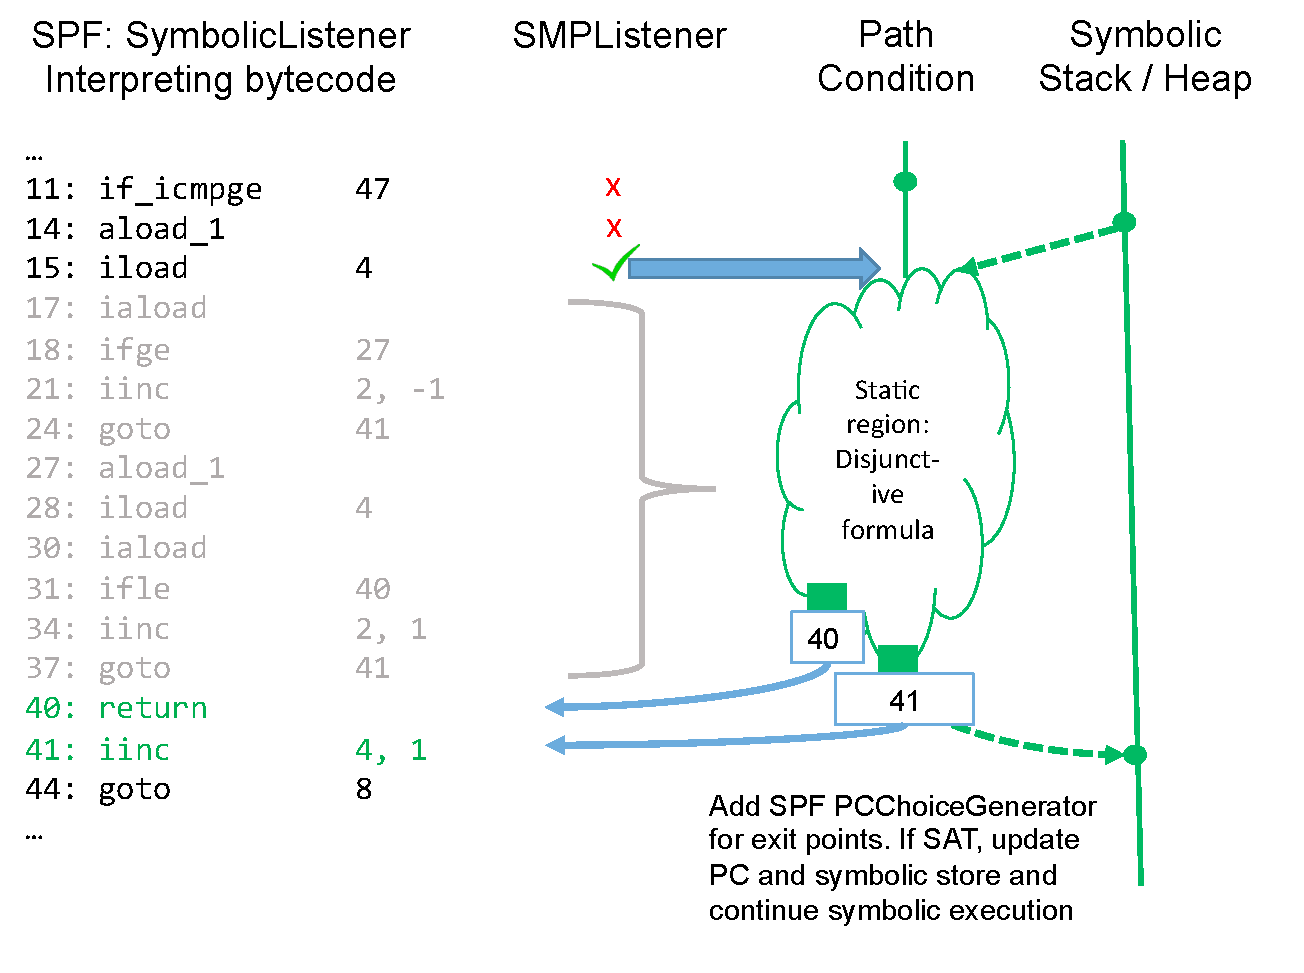
\includegraphics[width=\columnwidth]{figures/spf_veritesting}
\end{figure}


\section{Related Work}
%Talk about veritesting in Mayhem, Angr.
%
The original idea for veritesting was presented by Avgerinos et al.~\cite{veritesting}.
%
They implemented veritesting on top of MAYHEM~\cite{mayhem}, a system for finding bugs at the X86 binary level which uses symbolic execution.
%
Their implementation demonstrated dramatic performance improvements and allowed them to find more bugs, and have better node and path coverage.
%
Veritesting has also been integrated with another binary level symbolic execution engine named {\tt angr}~\cite{angr}.
%
Veritesting was added to {\tt angr} with similar goals of statically and selectively merging paths to mitigate path explosion.
%
However, path merging from veritesting integration with {\tt angr} caused complex expressions to be introduced which overloaded the constraint solver.
%
Using the Green~\cite{green} solver may alleviate such problems when implementing veritesting with SPF.
%
Another technique named \textit{MultiSE} for merging symbolic execution states incrementally
was proposed by Sen et al.~\cite{multise}.
%
MultiSE computes a set of guarded symbolic expressions for every
assignment and does not require identification of points where
previously forked dynamic symbolic executors need to be merged.
%
MultiSE complements predicate construction for multi-path regions beyond
standard exit points~(such as
\textit{invokevirtual},~\textit{invokeinterface},~\textit{return}
statements).
%
Combining both techniques, while a substantial implementation effort, has the potential
to amplify the benefits from both techniques.
%This observation became even more apparent for longer paths.
%
%Integrating veritesting with SPF may expose a similar trade-off.
%
%But we expect this problem to be less severe for when doing static symbolic execution of Java bytecode because Java bytecode instructions have fewer behaviors to be statically analyzed than X86 architecture instructions.

% %Talk about other symbolic execution performance improvements.
% %mentioned in Christopher Kruegel's ISSTA keynote talk as Static Analysis support
% Other static analysis techniques also provide support for dynamic symbolic execution.
% %
% Loop-extended symbolic execution introduced partial loop summarization by having symbolic variables that represent the number of times each loop executes.
% %
% This technique allowed symbolic variables to incorporate loop dependent effects along with data dependencies from program inputs.
%
%Value Set Analysis~\cite{vsa} is another static analysis technique that can potentially benefit dynamic symbolic execution.
%%
%Value set analysis uses an abstract domain to find an over-approximated set of values that registers or abstract locations may have at program points.
%%
%Value set analysis can help dynamic symbolic execution resolve ranges without solving constraints.
%VSA can resolve ranges without solving constraints, thereby, finding applications in computing all possible write targets during a memory write operation.
%Code summarization (Dodo)
%  - automatically (and statically) summarize effect of loops / functions
%VSA - value set analysis
%  - resolve ranges (and conditionals) without solving constraints

%Talk about TamiFlex, and how using the same technique as TamiFlex is one way to solve veritesting challenges in Java bytecode.
%
%Other techniques for static analysis at the Java bytecode level can also benefit dynamic symbolic execution.
%
Finding which reflective method call is being used, or handling dynamic class loading are known problems for static analysis tools.
%
TamiFlex~\cite{tamiflex} provides an answer that is sound with respect to a set of previously seen program runs.
%
Integrating veritesting runs into similar problems, and using techniques from TamiFlex would allow static predicate construction beyond exit points caused by reflection or dynamic class loading. 

\section{Conclusion}
%Talk about veritesting is important, but implementing it at the Java bytecode requires solving different research and engineering challenges.
Veritesting provides a way to address the scalability challenges faced by dynamic symbolic execution.
%
But, integrating veritesting with symbolic execution at the Java bytecode level presents unique challenges.
%
Our Soot-based analysis of six large open-source Java projects confirms that, while a number of opportunities to apply veritesting arise organically in Java bytecode, the benefit of veritesting can be amplified further by incorporating static symbolic execution of virtual function invocations and reducing the number of exit points introduced by exceptions and early return statements.
%
Implementing veritesting with the Symbolic PathFinder motivates robust implementation of expression reuse and introduction of complex expressions.
%
Using veritesting to its full extent during symbolic execution of Java bytecode requires us to address such research and engineering challenges.
%
But, veritesting has clear potential to provide significant speed-up to symbolic execution tools such as Symbolic PathFinder.

\section{Acknowledgements}
We would like to thank the Google Summer of Code program for supporting this research. 
%
This material is based upon work supported by the National Science Foundation under Grant Number 1563920.


\bibliographystyle{ACM-Reference-Format}
\bibliography{references}

\end{document}
